\documentclass[zihao=-4]{ctexart} % 全局字号设为小四号

% ========== 基本宏包 ==========
\usepackage{xeCJK} % 支持中文
\usepackage{setspace} % 设置行距
\usepackage{multirow} % 支持表格单元格跨行
\usepackage{titlesec} % 自定义标题格式
\usepackage{fancyhdr} % 自定义页眉页脚
\usepackage{indentfirst} % 让第一段也有首行缩进
\usepackage[a4paper, margin=1in]{geometry} % 设置页面布局
\usepackage{lipsum} % 生成示例文本(可移除)
\usepackage[colorlinks=true, linkcolor=black, anchorcolor=blue, citecolor=blue]{hyperref} % 生成 PDF 书签
\usepackage{graphicx} % 支持图形和表格调整
\usepackage{array} % 支持表格列格式调整
\usepackage{amsmath} % 支持数学公式对齐
\usepackage{physics} % 物理符号宏包
\usepackage{siunitx} % 单位符号宏包
\usepackage{tabularray} % 表格宏包
\usepackage{enumitem} % 用于自定义列表格式
% 设置段首缩进
\setlength{\parindent}{2em} % 设置段首缩进为 2 个字符宽度

% ========== 字体配置 ==========
\setCJKmainfont{SimSun}[ % 全局中文字体为宋体
   BoldFont = SimSun,   % 中文粗体用宋体
   ItalicFont = KaiTi,   % 中文斜体用楷体
   Scale=1.0             % 确保字体大小与字号匹配
]
\setmainfont{Times New Roman} % 英文字体为 Times New Roman
%自定义宋体加粗命令
\newcommand{\boldSun}{\CJKfontspec[FakeBold=3]{SimSun}}

% ========== 行距配置 ==========
\setstretch{1.25} % 设置正文行距为 1.25 倍

% ========== 标题格式 ==========
% 一级标题格式:三号宋体加粗,带中文编号
\titleformat{\section}
  {\zihao{-3}\boldSun} % 标题字体为宋体,模拟加粗
  {\chinese{section}、} % 标题编号格式:X、
  {0.5em} % 编号与标题内容的间距
  {} % 标题前缀

% 二级标题格式:四号宋体加粗
\titleformat{\subsection}
  {\zihao{4}\boldSun} % 标题字体为宋体,模拟加粗
  {} % 不显示编号
  {0em} % 编号与标题内容的间距
  {}
%三级标题格式:小四号宋体
\titleformat{\subsubsection}
    {\zihao{-4}\boldSun} % 小四号字体
    {} % 不显示编号
    {0em} % 编号与标题内容的间距
    {}

% 标题间距设置
\titlespacing*{\section}
  {0pt} % 左缩进
  {0.3\baselineskip} % 上方间距
  {0.3\baselineskip} % 下方间距

\titlespacing*{\subsection}
    {5pt}
    {0.3\baselineskip}
    {0.3\baselineskip}
\titlespacing*{\subsubsection}
    {7.5pt}
    {0.3\baselineskip}
    {0.3\baselineskip}
% ========== 页眉页脚 ==========
\pagestyle{fancy}
\fancyhf{} % 清空默认页眉页脚
\fancyhead{} % 确保页眉清空
\fancyfoot{} % 确保页脚清空
\fancyfoot[C]{\thepage} % 页脚居中显示页码
\renewcommand{\headrulewidth}{0pt} % 去掉页眉下划线
\renewcommand{\footrulewidth}{0pt} % 去掉页脚上划线

% ========== 自定义标题 ==========
\title{实验五\quad 时序逻辑电路}
\author{JS124620\quad 高越}
\date{\today} % 使用当前日期
\makeatletter
% 修改 \@title 的行为
\renewcommand{\maketitle}{
    \begin{center}
        {\zihao{2}\CJKfontspec[FakeBold=3]{SimSun} \@title} \\[0.75em] % 标题为二号宋体加粗
        {\zihao{-4} \@author} \\[0.5em] % 作者为 large 字号
        {\zihao{-4} \@date} % 日期为 small 字号
    \end{center}
}
\makeatother

\begin{document}\zihao{-4}
\maketitle % 显式设置正文为小四号

\section{实验内容} % 自动编号
设计一个只有小时和分钟功能的简易数字钟,输入时钟脉冲的周期为1分钟,4位数码管用于显示,高
2位显示小时($0\sim 23$),低2位显示“分钟”($0\sim 59$)。

(1) 设计并搭试电路,验证电路结果

(2) 用双踪示波器观察并记录“分钟”计数电路中的时钟脉冲及计数器的各输出波形

(3) 用双踪示波器观察并记录“小时”计数电路中的时钟脉冲及计数器的各输出波形
\section{实验设计方案}
\subsection{设计思路}
本实验设计一个简易数字钟,主要由计数器和数码管显示器组成。计数器用于计时,数码管用于显示时间。计数器部分可分为以下三个模块:

    (1) 模60计数器,用于分钟计数。

    (2) 模24计数器,用于小时计数。

    (3) 组合逻辑电路,用于根据产生进位和置数的控制信号。

模60计数器内中包含一个模10计数器和一个模6计数器可分别用模16计数器$U_0$和$U_1$实现,模24计数器内包含一个模10计数器和一个模3计数器分别用模16计数器$U_2$$U_3$实现。这四个部分均可以用同步置数法实现,即在满足一定条件时用置数功能将计数器各输出位全部置0。
各个模块之间连接时,低位向高位发出进位信号。
\subsection{进位和置数信号产生的条件}
为了设计出产生进位和置数信号的组合逻辑电路,需要列出各个模16计数器递增和置数的条件。假设该简易电子钟从高位到低位对应的十进制数分别是$Q_3Q_2Q_1Q_0$,则$U_0$$U_1$$U_2$$U_3$四个计数器递增及置数的条件如表\ref{tab:condition}所示。当满足递增条件时,组合逻辑电路应向计数器的使能端输出高电平,使计数器输出递增;当满足置数条件时,组合逻辑电路应向计数器的$\overline{LOAD}$端输出低电平,使计数器输出置零。
\begin{table}[h]
    \centering
    \begin{tblr}{|*{3}{Q[c,m,11em]|}}
        \hline
        计数器 & 递增条件 & 置数条件  \\ \hline
        $U_0$ & - & $Q_0=9$  \\ \hline
        $U_1$ & $Q_0=9$ & $Q_1Q_0=59$  \\ \hline
        $U_2$ & $Q_1Q_0=59$  & $Q_2Q_1Q_0=959$或$Q_3Q_2Q_1Q_0=2359$ \\ \hline
        $U_3$ & $Q_2Q_1Q_0=959$ & $Q_3Q_2Q_1Q_0=2359$  \\ \hline
    \end{tblr}
    \caption{进位信号及置数条件}
    \label{tab:condition}
    \end{table}
    根据这些条件,不难设计出能正确产生进位和置数信号的组合逻辑电路。
\subsection{逻辑电路图}
跟据设计思路及位和置数信号产生的条件,不难画出简易电子钟的逻辑电路图如图\ref{fig:logic}所示。使用MultiSim软件对该电路图的功能进行验证,该电路能够实现题目所要求的功能。
\begin{figure}[htbp!]
    \centering
    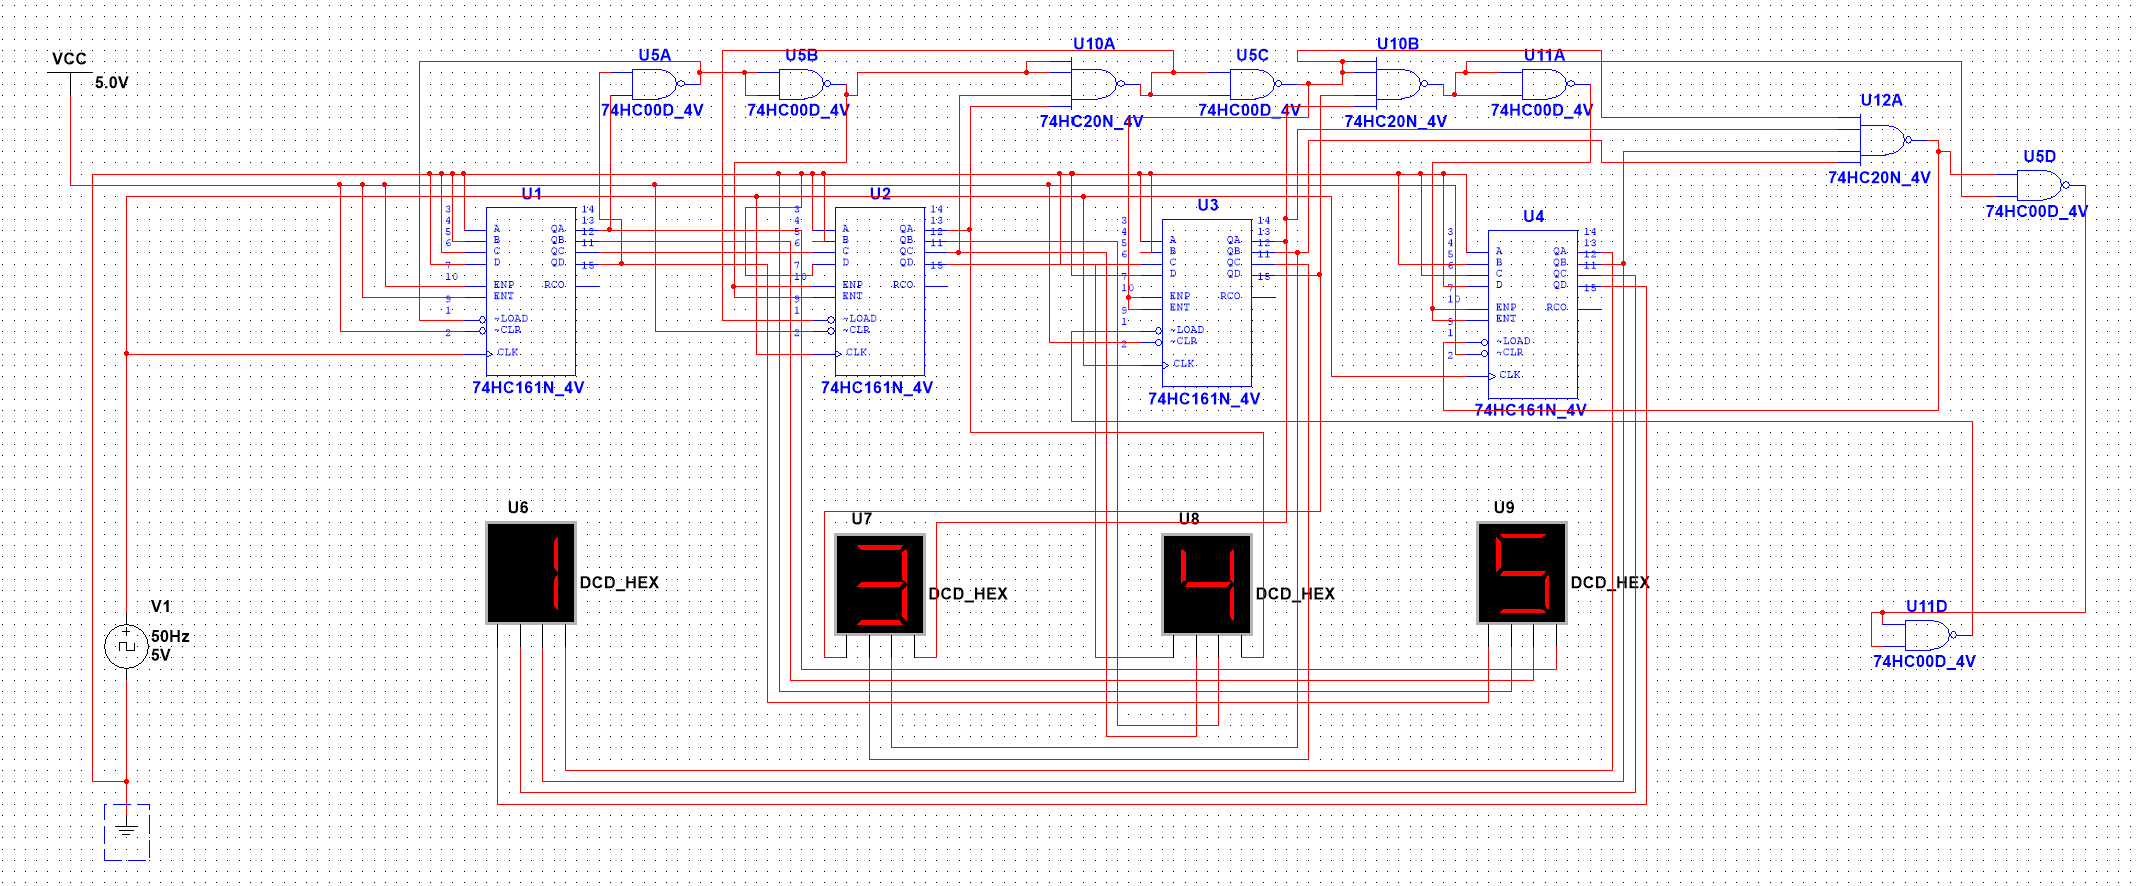
\includegraphics[width=1\textwidth]{../img/Lab5_Ex3.png} % 确保文件名和路径正确
    \caption{简易电子钟逻辑电路图}
    \label{fig:logic}
  \end{figure}
\section{测试方案}
(1) 将时钟脉冲信号接入电路,电路输出接入四位数码管,验证电路功能。

(2) 用双踪示波器观察并记录“分钟”计数电路中的时钟脉冲及计数器的各输出波形。

(3) 用双踪示波器观察并记录“小时”计数电路中的时钟脉冲及计数器的各输出波形。
\end{document}